% Doc class required by class assignment.
\documentclass{sig-alternate-05-2015}

% copyright and other misc things provided by template.
% DOI
\doi{10.475/123_4}

% ISBN
\isbn{123-4567-24-567/08/06}

%Conference
\conferenceinfo{PLDI '13}{June 16--19, 2013, Seattle, WA, USA}

\acmPrice{\$15.00}
% end copyright
\begin{document}

% Paper title
\title{CSC 510 Software Engineering: Project 1 
    %\titlenote{(Paper 1). For use with
    %SIG-ALTERNATE.CLS. Supported by ACM.}
}
\subtitle{Group-P
%\titlenote{A full version of this paper is available as
%        \textit{Author's Guide to Preparing ACM SIG Proceedings Using
%        \LaTeX$2_\epsilon$\ and BibTeX} at
%        \texttt{www.acm.org/eaddress.htm}
%    }
}

\numberofauthors{8} %  in this sample file, there are a *total*
\author{
% TODO: Fill Bikram's name properly
% TODO: Fill in addresses
\alignauthor
	Monica Metro %\titlenote{Dr.~Trovato insisted his name be first.}\\
       \affaddr{North Carolina State University}\\
       \affaddr{1932 Wallamaloo Lane}\\
       \affaddr{Wallamaloo, New Zealand}\\
       \email{mgmetro@ncsu.edu}
% 2nd. author
\alignauthor
	Zachery DeLong %\titlenote{Dr.~Trovato insisted his name be first.}\\
       \affaddr{North Carolina State University}\\
       \affaddr{2305 Horizon Hike Ct}\\
       \affaddr{Raleigh, NC}\\
       \email{zpdelong@ncsu.edu }
% 3rd. author
\alignauthor 
	Zhangqi Zha %\titlenote{Dr.~Trovato insisted his name be first.}\\
       \affaddr{North Carolina State University}\\
       \affaddr{1800 Vienna Wood Dr}\\
       \affaddr{Raleigh, NC}\\
       \email{zzha@ncsu.edu}
\and  % use '\and' if you need 'another row' of author names
% 4th. author
\alignauthor 
	Bikram\\
       \affaddr{Brookhaven Laboratories}\\
       \affaddr{Brookhaven National Lab}\\
       \affaddr{P.O. Box 5000}\\
       \email{bikram@ncsu.edu}
}
% Generate page header.
\maketitle


% Paper body
% Please do not delete!  thanks! -- zach
% !TEX root = ../main.tex

\begin{abstract}
  Choosing a textbook for a class is something that many professors do
  several times a year, but the vast number of available textbooks for
  any given subject makes choosing one that both meets the needs of
  the class and meets the budget constraints of today's students is a challenge.  
  In this paper, we propose two methods for automatically learning
  topics from books, a set of evaluations for those methods, and a
  system that will use those methods in a web app that attempts to
  suggest textbooks to a professor balancing covering all topics the
  course requires while still being economical for students.  
\end{abstract}

% Please do not delete!  thanks! -- zach
% !TEX root = ../../main.tex

\subsection{Background}
One of the most basic tasks that a professor must do is identify what textbook to use for a given class.
While some fields have textbooks that have become popular and are
clearly the best in their subject matter, many fields (especially
emerging ones) have no such exemplar and reading through all possible
candidates would be too time consuming to be feasible.  
It would be a complex enough problem if there were not already a
massive number of textbooks on sources such as Amazon, but self aware
professors have attempted to use textbooks that are less expensive
with hopes of allowing lower income students to attend more easily.  
This admirable intention serves to increase the already considerable
time needed to find appropriate books, and there is no obvious
heuristic to apply to searches to limit the field.  

In the interests of making students lives less expensive, have 
expored a system which can identify topics in books automatically, and
which, given a set of requirements from a user (our intention is for
the system to be used by a professor, but others may find value in it),
can suggest options of varying expense and completeness for a given set of topics.  
To do this, we propose exploring word clusters generated by Doc2Vec, a
family of common natural language processing (NLP) algorithms that
attempt to cluster similar words, and topics generated by latent
dirichlet allocation (LDA), another common NLP algorithm that directly
attempts  to identify topics in text, to automatically infer the
content of a set of textbooks.  

We then intend to build a web app that will allow a user to specify a
set of topics and which will use the mentioned algorithms to make
suggestions while minimizing the cost of said textbooks.  
The actual web app will be a fairly simple single-page web app
developed in Angular4 and using Bootstrap to hasten development of a modern UI.  

The team begain this experiment somewhat biased toward LDA as the
algorithm expected to perform, and this initial bias turned out to be
more or less correct.
After spending significant time training and validating a useful
Doc2Vec model, the team was unable to build a useful topic mining
algorithm on top of Doc2Vec.

%%% Local Variables:
%%% mode: latex
%%% TeX-master: "../../main"
%%% End:


\subsection{Deviations From Initial Plan}
\label{sec:devi-from-init-pln}

\subsection{Planning}
\label{sec:planning}

\paragraph{The Spiral Model}
\label{sec:spiral-model}

\paragraph{Prototypes}
\label{sec:prototypes}

% Please do not delete!  thanks! -- zach
% !TEX root = ../../main.tex

\section{Literature Review} \label{section:algorithms}
We propose two methods for analyzing and storing topics from books automatically: LDA and Doc2vec. 

\subsection{LDA}
\par In this section, we describe the Latent Dirichlet allocation(LDA) method for storing topics against books. 
\par LDA uses a Bayesian clustering approach to find topics relevant to the book. \cite{RefWorks:doc:5a721fb5e4b0d609eec83aa1} The input to the method is a book (or later, a series of books) which consists of collection of words. 
\par This method assumes that each book (or books) consists of topics and that each topic has several key words associated with it. The number of topics associated with a book can be variable, and can be changed for better optimization. In this association, words are the measurable variable whereas the topics are "latent" variables, that is they are not directly measurable but indirectly observed. 
\par The performance of the method depends on the initial assumptions made. For example, some have assumed that books are random mixes of topics \cite{RefWorks:doc:5a721e4ae4b095066af57410}. The number of topics can initally be chosen as constant for a given book, or as a function of a chosen Poisson distribution. \cite{RefWorks:doc:5a721e4ae4b095066af57410} Topic distribution in the book is assumed to be a sparse Dirichlet function.
\par A sparse Dirichlet function implies that we assume that a topic will be discussed only in a small breadth of pages in the book, and also that words relating to this topic will predominantly figure in these pages.
\par The algorithm looks to identify unique words to identify as topic names. Words like "the" and "a" are common and will occur with equal probability throughout the text. However, in say one chapter of the book some words may occur much more frequently in that particular chapter than the rest of the book, which means that the probability of these words in that chapter is more, which then the algorithm can use to choose a topic name and also a list of words related to that topic.

% This algorithm seems to be the clear winner.  

% Conceptually, this algorithm one-hot-encodes its input like Doc2vec does

% It then uses prior probabilities to identify words that are commonly paired with the given word.

% Through repeated training on the same data set, it will gradually identify topics among related text.

\subsection{Doc2Vec}
Doc2Vec is a model that extends an existing model, Word2Vec. Doc2vec mirrors Word2Vec in most ways except that it adds context information. \cite{RefWorks:doc:5a6e5748e4b0d609eec798dd}
% I'm not sure this algorithm really fits and shouldn't be replaced with something like LSI... see notes.  

% conceptually, this algorithm takes in a one-hot encoded vector and attempts to train a two-layer neural network to predict words around n-grams given.

% After iterations of training, it will give you a cluster of words that are similar to the given word.

% I guess we'd have to put something on top of Doc2Vec to use it for topic modeling.  I'm not entirely clear on how we'd do that.

% Not sure if the text below is 100% correct. Tried my best -M

	Doc2Vec is an implementation of the Paragraph Vector (PV) introduced by Mikolov and Le in 2014 - an unsupervised algorithm that generates vector representations of text. \cite{RefWorks:doc:5a6e5746e4b0d609eec798d7}  The basic difference between LDA and Doc2Vec is that LDA tries to form a structure of related words (a topic name with the list of associated words) out of books mainly on the basis of frequency of words in the document. While a simple yet powerful approach, it has a few drawbacks, such as semantics. For example, the words "powerful, strong and Paris" are equally distant when considered by a bag of words model, however "powerful" and "strong" are semantically close. \cite{RefWorks:doc:5a6e5746e4b0d609eec798d7}
	
	Paragraph Vector invloves predicting words in the paragraph. It is "unsupervised", which means that it predicts words in a paragraph and then uses these predictions to attempt to form structures of related words without any knowing of accuracy of the structure(s). The PV utilizes fixed length feature vectors learned from text sources of variable length.
	
	Mikolov offers two models of PV that are based on the implementation of Word2Vec: Distributed Memory Model (PV-DM) and Distributed Bag of Words (PV-DBOW).

%I would like to talk more about unsupervised algorithms and clustering but i don't quite understand it

PV-DM is similar to the Continuous Bag of Words (CBOW) model in Word2Vec such that is predicts the next word based on the given context. Paragraph vectors are concatenated with word vectors from that paragraph.  Each word vector is representing a word from the given context and a new vector is generated by concatenating all of those word vectors together to predict other words. These word vectors are able to remember context and semantics. The paragraph vector allows the algorithm to remember the topic or 'label' of the paragraph, whether it is a sentence or a long document. 
% This is an advantage over the traditional Bag of Words model which does not account for either resulting in each word having the same amount of weight to each other. Consequently similar words are not mapped close together. 

PV-DBOW follows the skip-gram model of Word2Vec. In this model, instead of concatenating the paragraph vector with the word vectors formed in close proximity in order to predict the next word, random text from the paragraph is selected and a random word is selected from that text. Because this model does not save the word vectors and therefore does not retain as much information about the context and semantics of the text, it requires less storage.


\subsection{Related Work}
%Planning on talking about that twitter article at the very least, and a little about the recommendations made by Mikolv for Doc


% Please do not delete!  thanks! -- zach
% !TEX root = ../../main.tex

\section{Proposed Solution} 
To tackle this problem, we propose a three-part system that will go about recommending books via a web app.  
The first component of this system is a recommendation engine, which will implement the above algorithms in some way and store their results (the topics) in an indexed database which we can summarily search.  
The next component will be a recommendation engine which will implement our recommendation algorithm (see below for more details).  
The third component will be a web app that will allow the end-user to search the database of topics and organize them into a useful search of books.  
It will then present a list of suggested books using the infrastructure mentioned earlier.  

\subsection{Book parser} \label{section:book-parser}
% Please do not delete!  thanks! -- zach
% !TEX root = ../../main.tex

The first major component of the system is the book parser.  
We intend to implement this taking advantage of the pre-built libraries available in Python such as SKLearn, Pandas, and others.  
The goal of the book parser is to implement one of the two algorithms discussed in section \ref{section:algorithms} and to store the parsed topics in a database for searching later.  
This will be implemented using the command pattern, which provides a simple interface to implementing different algorithms in code and allows us to easily swap between implementations.



% TODO: Can we decide on a few and list them here somehow?
The books being parsed will come from a freely available online database of textbooks.  
We have found a number of websites such as openstax.org and onlinebooks.library.upenn.edu that offer free libraries of textbooks that we are evaluating for use for this project.
It is our intention to use a REST API or something similar to poll for books to analyze.

We are also exploring how much of the books we need to parse.
Parsing entire books for topics is infeasible as the number of books grows (and as our introduction pointed out, there are plenty of books to parse) but we need to ensure that we have enough text to encapsulate all of the important topics the books cover, and that we have enough text to reliably train our algorithms on.
To test this, the team intends to do testing before we test the actual application to see how much training is required when parsing the table of contents only, the index only, and any available summaries.
We also intend to test some combinations such as the table of contents and the index together, to try to isolate what section might be most useful for training.


Because analyzing entire libraries of books is not something that we can do in real time, we plan to cache the topics parsed from these algorithms in a database to be referenced in the future.  
We are evaluating MySQL, Postgress, and an object-oriented DB such as Mongo for this task.  
This will allow us to train the algorithms on the books ahead of time and will make searching for books based on topics much more efficient. 
It also allows us to do routine similarity analysis on the topics of books to identify potential synonyms between topics.
In other words, we could store the topics from two different books in the same database tables we are exploring algorithms that might then allow us to identify similarities in topics mined and then link the books to the same topics for future analysis.  
That said, this is a very lofty goal in an already complex project, and similarity analysis may need to be cut for time constraints.

\subsection{Recommendation Engine} \label{section:recommendation_engine}
% Please do not delete!  thanks! -- zach
% !TEX root = ../../main.tex

The next step in our problem is to use the topic analysis data outlined in the previous section (\ref{section:book-parser}) to suggest books based on the topics covered and the cost.
This algorithm will be written in Python as well.  

Conceptually, this algorithm will need to take in a set of required topics and weighting for topics vs price.
This value will be used to favor inexpensive books over complete topic coverage in our algorithm.
It will then search its algorithms for books that meet the required topics.
The algorithm should then rank the books using the weighting mentioned earlier, then it will sort some number of the top results and give them back to the UI.

\subsection{Web App} \label{section:webapp}
% Please do not delete!  thanks! -- zach
% !TEX root = ../../main.tex

The web app is the final component of this architecture and it serves to tie the previous two components together.
The app provides the UI to the algorithms, allowing professors to log in and select a set of subjects they wish to teach on, then it should present them with a UI for searching for topics in our database.  
It should then allow them to create a list of topics to suggest books for.
Once the list has been generated, the tool should search against the book databases it has access to using the algorithms outlined in the previous sections.

We will develop this app in either the MEAN stack or some variant thereof.  (Does it make more sense to just use Django since we are writing learning algorithms in Python?)
The front-end will be developed using Bootstrap to save time in developing a useful, mobile friendly UI.
In the end, the app itself will be a single-page web app that includes minimal authentication features.  
The real complexity of this app is in the learning algorithms and the suggestion engine, so the front end of the app itself needs only to be a client to reach out to those algorithms.  


% Please do not delete!  thanks! -- zach
% !TEX root = ../../main.tex

\section{Evaluation Plan}
In this section, we will talk about methods to evaluate our solutions. This including two parts: methods used to evaluate our topic learning model and methods used to evaluating textbook suggestions which is our final product. 

\subsection{Evaluating Topic Modeling}
In order to carry out a comparative evaluation for a set of candidate recommendation algorithms, evaluation metrics will be used to measure some quality and performance features, in our case, we will use prediction accuracy to evaluate the models. The most popular metric that is used for evaluating prediction accuracy is Root Mean Squared Error (RMSE). RMSE is used measure of the differences between values (sample and population values) predicted by a model or an estimator and the values actually observed.  We will need to run this RMSE analysis on a data set with labels, and we are currently evaluating available data sets on Kaggle for fitness for this task.  
\newline
\begin{equation}
   RMSE = \sqrt{\frac{\sum_{1}^{n}\left ( \widehat{y_i}-y_i \right )^{2}}{n}}
\end{equation}
   
%i.	Surveying?
%ii.	Build a UI to present a book and a topic that was thought to be in the book
%iii.	User validates yes/no
%iv.	We use that feedback to tweak parameters of our models and to identify how many iterations of training we need to do (both our algorithms improve with more iterations)
\subsection{Evaluating textbook suggestions}
\subsubsection{Pre-Surveying}
To evaluate our project idea, we conducted a pre-surveying to see what the problem we are facing and how people reacting about our proposed solution. We asked our participants how long they will spend on find the right textbook, what aspect do they think is most important when choosing a textbook (except the content, our learning model will do the best of this part). See Table \ref{Pre-survey} for a breakdown of the questions to ask.

\begin{table}[ht] 
\caption{Questions in Pre-survey}
\label{Pre-survey}
\begin{center}
\begin{tabular}{ll}
\multicolumn{1}{c}{\bf Questions} 
\\ \hline \\
1. Are you a student or professor?\\
2. How much time do you spend on choosing a textbook?\\
3. How do you choose a textbook?\\
4. What aspect do you think is most important\\
when choosing a textbook (except the content)? \\
5. Would you consider an app that will give you \\
recommended textbooks base on your course \\
syllabus and your preference? \\
\end{tabular}
\end{center}
\end{table}
Among the 29 responses, we found that 73.3\% responded as they interested to our application to recommend the textbooks. The answer to most important aspect during the textbook chosen, review/ratings and sell price were the highest concern. These preliminary results give us the guidance to design the application and to improve the core learning models. See Figure \ref{tesult_of_presurvey} for detail results.
% Hi Zach, could you please help me to add figure preSurvey.jpeg here? Thanks.

\begin{figure}[ht]
\caption{Result of preSurvey}
\centering
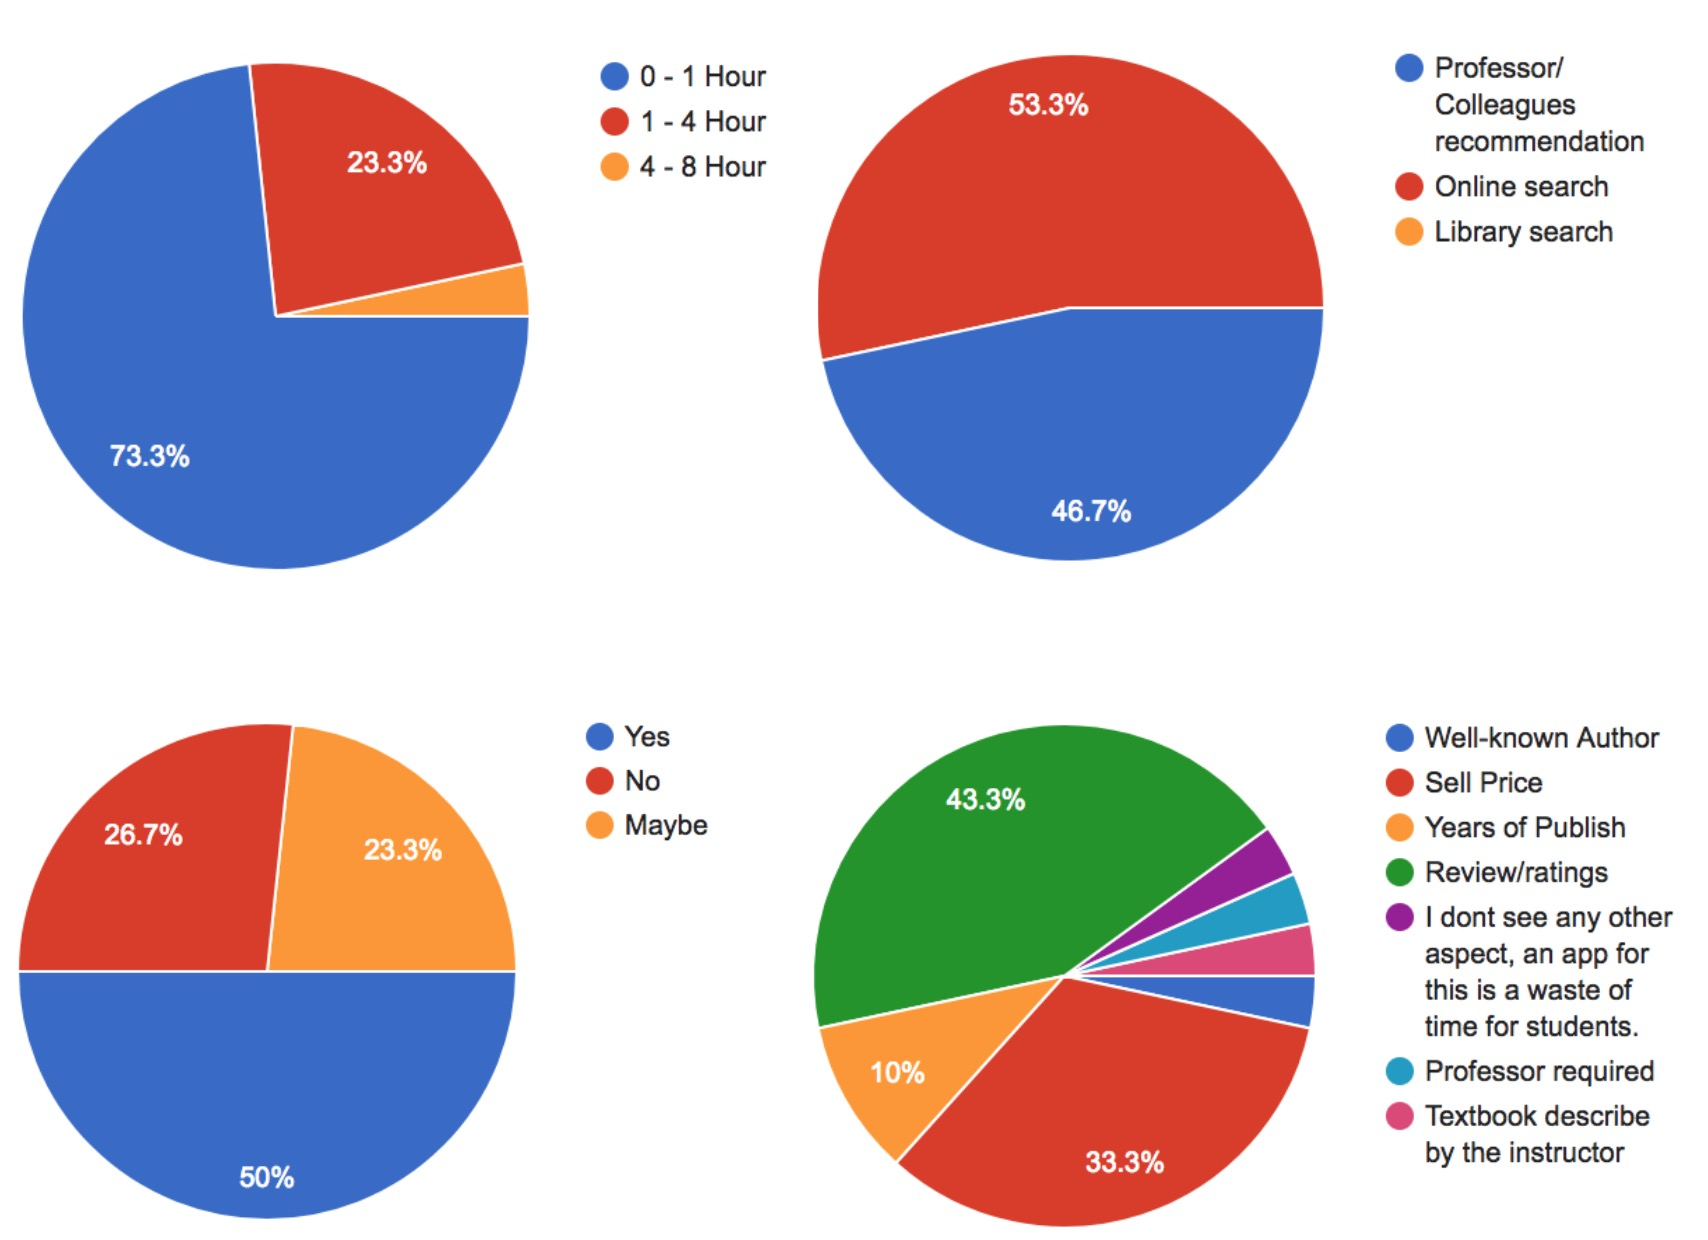
\includegraphics[width=0.5\textwidth]{preSurvey.jpeg}
\end{figure}
\subsubsection{Experiments and Post-survey}
After we build the application UI and core learning model, we plan to run a few experiments with different groups of users to evaluate the solution.

We have briefly discussed how we intend to validate that our model suggests books well and the usefulness of our application overall, but we have not yet discussed how we intend on validating whether or not the textbook recommendations that our algorithm make are topical (cover the topics) and are frugal (are less expensive than other options).  
To do this, we intend to do some focus grouping easier by some custom UI in our web app.

We intend to sit down a group of volunteers with our app and to give them access to our app with an anonymized user.  
They will be asked to find an appropriate textbook for a class using a provided list of topics.  
After choosing the appropriate topics and setting their own weighting on frugality and topic coverage, they will be asked to parse the results and rank their fitness for the particular purpose on a scale from $1$ to $5$ (with $5$ being perfect fit) and rate their cost from $1$ to $5$ (with $5$ being perfectly inexpensive compared to the alternatives).  
After rating the books that were suggested, the user will then be presented with the top 5 books that did not make the suggestion cut, and will be asked if any of these books should have replaced books that were presented and why they should have been on the list (for example, was the book expensive, but did it offer better topic coverage, or was there something unique about it that we should factor into our analysis).  
The test can then be repeated with the other algorithm.

This test will answer several questions.  
First, it allows us to evaluate if the topic mining is finding semantically appropriate items.  
By presenting the user with the top choices, then choices that were not considered optimal, we are attempting to see if the algorithm should have found a different book more relevant.  
We are also attempting to see if a book that was more or less expensive should have been on the list.  
More importantly, though, by rating suggestions on a 1 to 5 scale, we can easily compare the ratings of suggestions made by LDA to the ratings of suggestions made by Doc2Vec to see if there is a significant difference between them.  


%i.	Surveying?
%ii.	User selects topics they want to search for
%iii.	App presents 3 answers: 
%1.	an expensive but complete solution,
%2.	an inexpensive but incomplete solution,
%3.	a middle-of-the-road solution
%iv.	User identifies if the solutions are reasonable
%v.	User is presented with more (how many) books that did not make the cut, and is asked if one of those should have been in the top 3.  




% Please do not delete!  thanks! -- zach
% !TEX root = ../main.tex

\section{Conclusion}
\subsection{Anticipated challenges}
% We anticipate there being problems in setting up Doc2Vec
% We do not have NLP expertise on our group's staff, so we will need to consult with TAs and do extra research.  

\subsection{Tentative schedule}
% This section needs to provide a simple table with week breakdowns of tasks with the condition 
% that we are still planning and researching and the schedule will change.
\subsection{Future enhancement}
One major enhancement would be the introduction of a rating system to the suggestion engine.  
Another major enhancement would be including links in the UI to buy the books.
A third major enhancement would be evaluating other topic modeling algorithms to see how they stack up.
Another enhancement would be to test an even more rudimentary topic modeling method, such as simply representing topics as lines in a table of contents.  
Essentially asking the question of whether or not fancy algorithms are even more useful that simple text search for this domain.

% End paper body

% REMOVE NOCITE OR IT WILL LIST EVERYTHING IN YOUR DATABASE AS A REFERENCE
%\nocite{*}

% Bibliography/style
\bibliographystyle{abbrv}

\bibliography{export}
% End bibliography/style

\end{document}
